\documentclass{article}
\usepackage[utf8]{inputenc}
\usepackage{graphicx}
\usepackage{mathtools} 
\usepackage{textcomp}
\usepackage{titling}
\usepackage{subfig}
\usepackage{amsmath}
\usepackage[parfill]{parskip}
\usepackage{xcolor}
\definecolor{LightGray}{gray}{0.9}
\usepackage{titlesec}
\setcounter{secnumdepth}{4}
\usepackage[a4paper,left=1cm,right=1cm,top=1cm,bottom=1.5cm,]{geometry}
\usepackage{eqparbox}
\usepackage{enumitem}

\title{\vspace{-2cm} EE4218 L5 - HLS}
\date{\vspace{-5ex}}

\begin{document}
\maketitle

\section{Context}
Suppose we want to implement hardware for the code below.
\begin{figure}[htp]
    \centering
    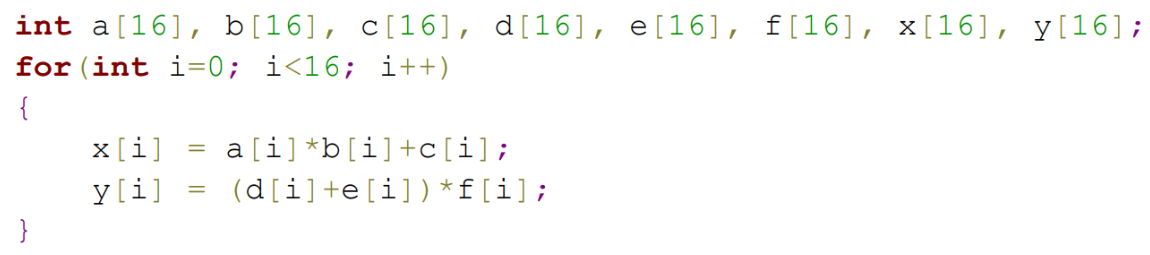
\includegraphics[width=12cm, scale=1]{S1/contextCode.PNG}
\end{figure}

Assume \dots
\begin{itemize}
    \item \textit{a[i]}'s to \textit{f[i]}'s are seperate memories that can be read asynchronously
    \item \textit{x[i]}'s and \textit{y[i]}'s are seperate memories that are written synchronously
    \item Adder has delay of 5ns, Multiplier has delay of 10ns
    \item Circuit is resource-dominated (ie. Area and performance depend on a few well-characterized functional resources)
\end{itemize}

\section{Single-cycle vs Multi-cycle design}
\subsection{Single Cycle}
Single cycle design is where all of the logic is done \textit{combinationally} in one cycle

\begin{minipage}[t]{0.5\textwidth}
    \vspace{0pt}
    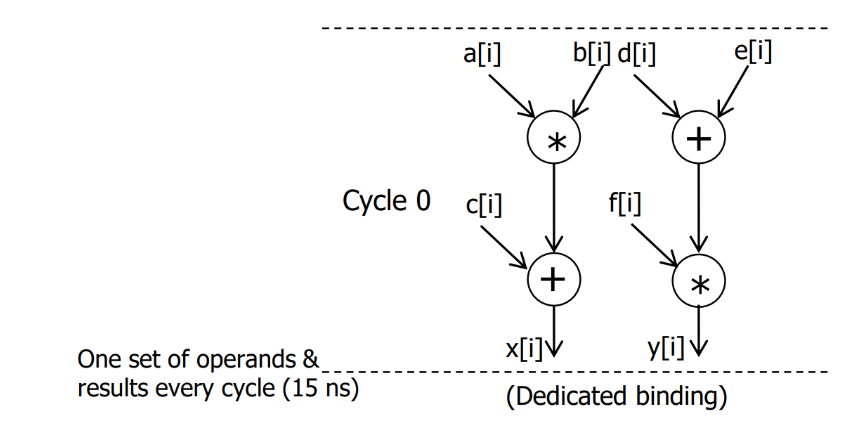
\includegraphics[width=9cm, scale=1]{S1/singleCycle_scheduling.PNG}
    \captionof{figure}{Single Cycle - Scheduling}
\end{minipage}%
\begin{minipage}[t]{0.5\textwidth}
    \vspace{0pt}
    Notice that scheduling is trivial, since all computations are done combinationally.
    Therfore, there is only a single time-step in the schedule. \newline

    Furthur note that no resource-sharing is possible, since all operations are done in the same cycle \newline

    \begin{itemize}
        \item 2 ALUs, 2 MULs
        \item Period = 15ns
        \item Latency (per iteration) = 1 cycle
        \item Trip Count (number of loop iterations) = 16
        \item Total latency = 16 cycles
    \end{itemize}
\end{minipage}

\begin{figure}[htp]
    \centering
    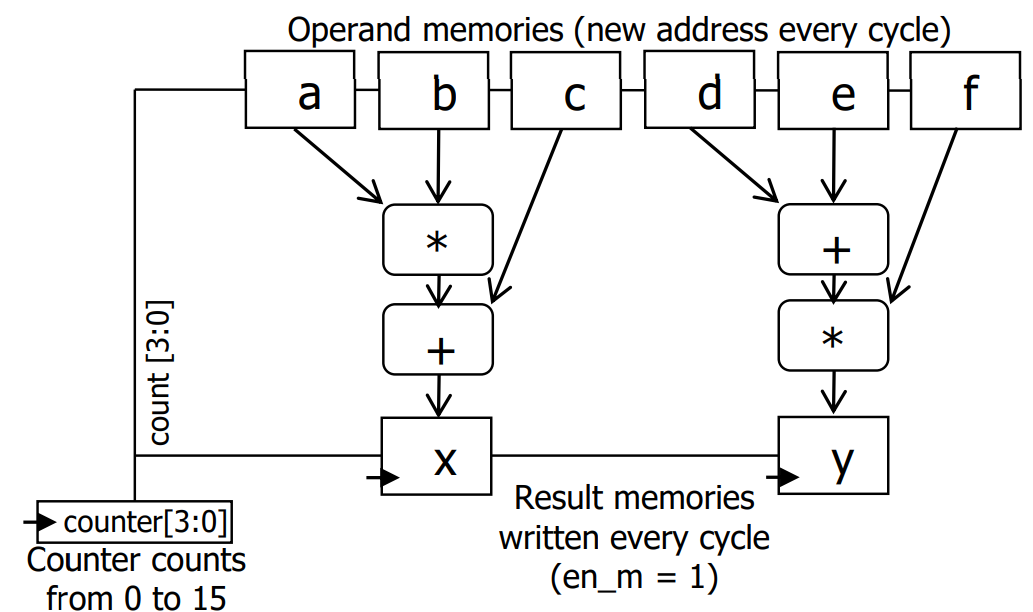
\includegraphics[width=12cm, scale=1]{S1/singleCycle_hardware.PNG}
    \caption{Single Cycle - Hardware implementation\\
            Note that \textit{counter} is an abstraction of our control logic}
\end{figure}

\subsection{Multi Cycle (default in older version of HLS)}

\begin{minipage}[t]{0.5\textwidth}
    \vspace{0pt}
    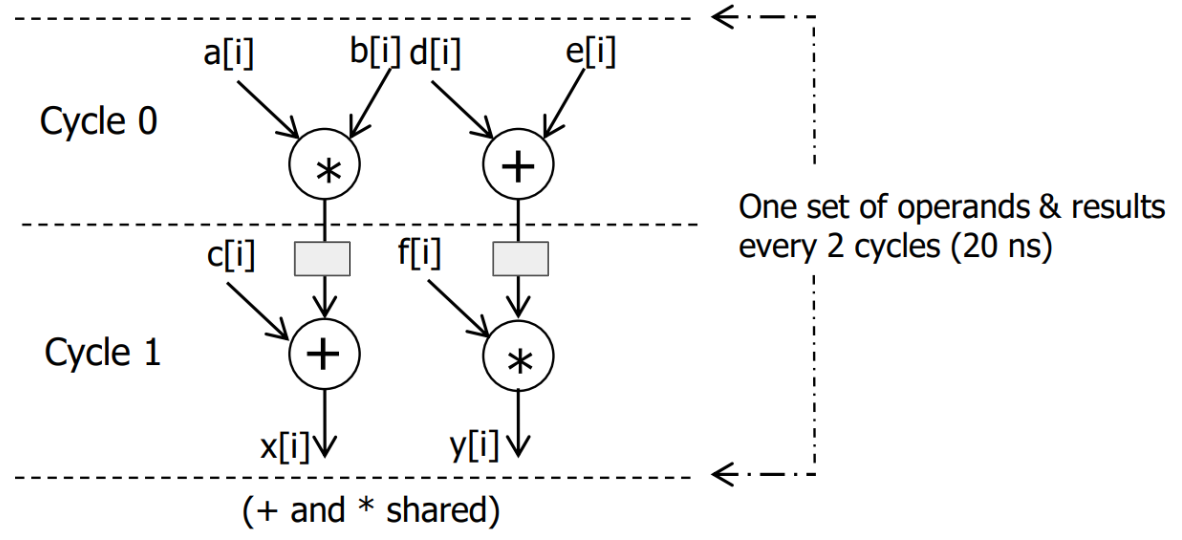
\includegraphics[width=9cm, scale=1]{S1/multiCycle_scheduling.PNG}
    \captionof{figure}{Multi Cycle - Scheduling}
\end{minipage}%
\begin{minipage}[t]{0.5\textwidth}
    \vspace{0pt}
    Note the inclusion of temp registers to store the intermediate results (with MUX \textit{sel} signals channeling it appropriately) \newline

    Resource-sharing is now possible, and the clock period (bounded by the slower MUL unit) is decreased as well \newline

    \begin{itemize}
        \item 1 ALU, 1 MULs
        \item Period = 10ns
        \item Latency (per iteration) = 2 cycle
        \item Trip Count (number of loop iterations) = 16
        \item Total latency = 32 cycles
    \end{itemize}
\end{minipage}

\begin{figure}[htp]
    \centering
    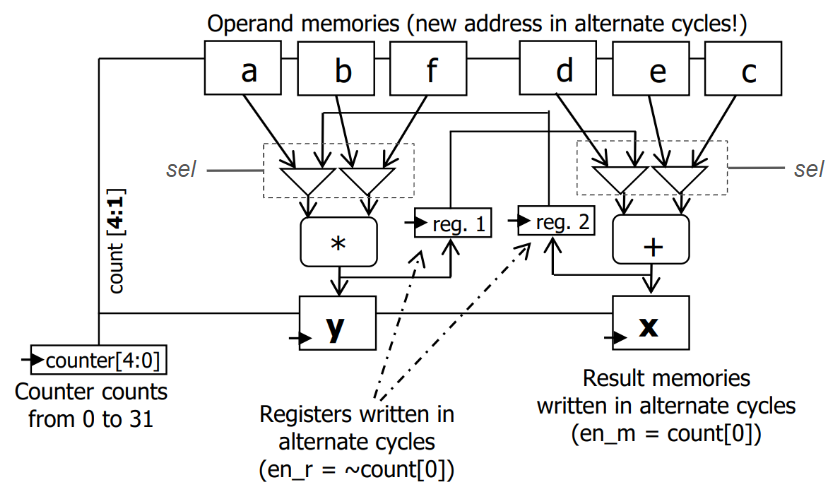
\includegraphics[width=12cm, scale=1]{S1/multiCycle_hardware.PNG}
    \caption{Multi Cycle - Hardware implementation}
\end{figure}

\section{Pipelining (default in newer version of HLS)}
In our multi-cycle design before, we had to complete the computation of the $i^{th}$ result before we could proceed to compute the $(i+1)^{th}$ result

Pipelining issues a new set of inputs every $j^{th}$ cycle instead, which we define as \textit{Initiation Interval}(II)

Therefore, the \textbf{absolute} latency per datapoint becomes less revelant, we are more interested in \textit{throughput} (datapoints processed per \textit{unit time})
\subsection{Pipelined (\textit{II = 1})}
Issuing a new set of inputs every cycle

\begin{minipage}[t]{0.5\textwidth}
    \vspace{0pt}
    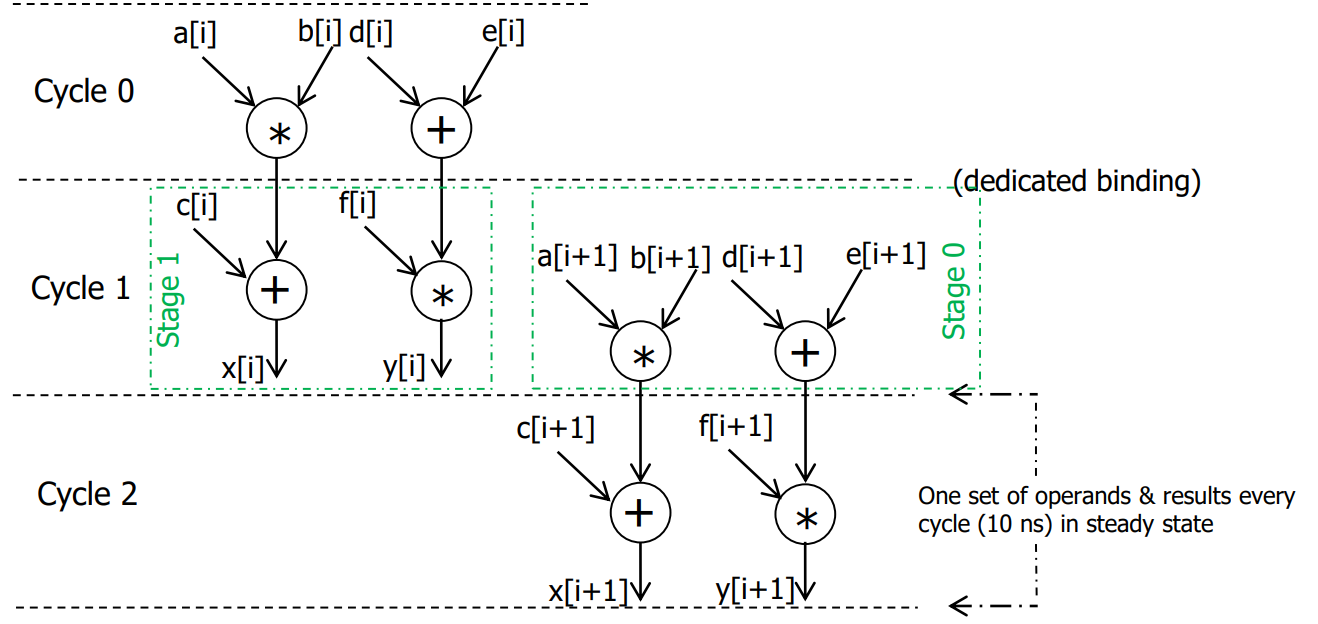
\includegraphics[width=9cm, scale=1]{S2/pipeline_II1_schedule.PNG}
    \captionof{figure}{Pipeline (II=1) - Scheduling}
\end{minipage}%
\begin{minipage}[t]{0.5\textwidth}
    \vspace{0pt}
    We implicitly assume the presence of temporary regs (to store data from $i^{th}$ to $(i^{th} + 1)$ cycle) \newline

    There is overlap in execution of the previous and current set of operands, 
    and at \textit{steady-state} we complete a computation at the end of every cycle \newline

    \begin{itemize}
        \item 2 ALUs, 2 MULs
        \item Period = 10ns
        \item Latency (per iteration) = 2 cycles
        \item Trip Count (number of loop iterations) = 16
        \item Total latency = (\textit{II} *tripCount) + 1 cycle overhead to fill pipeline = 17 cycles
    \end{itemize}
\end{minipage}

\begin{figure}[htp]
    \centering
    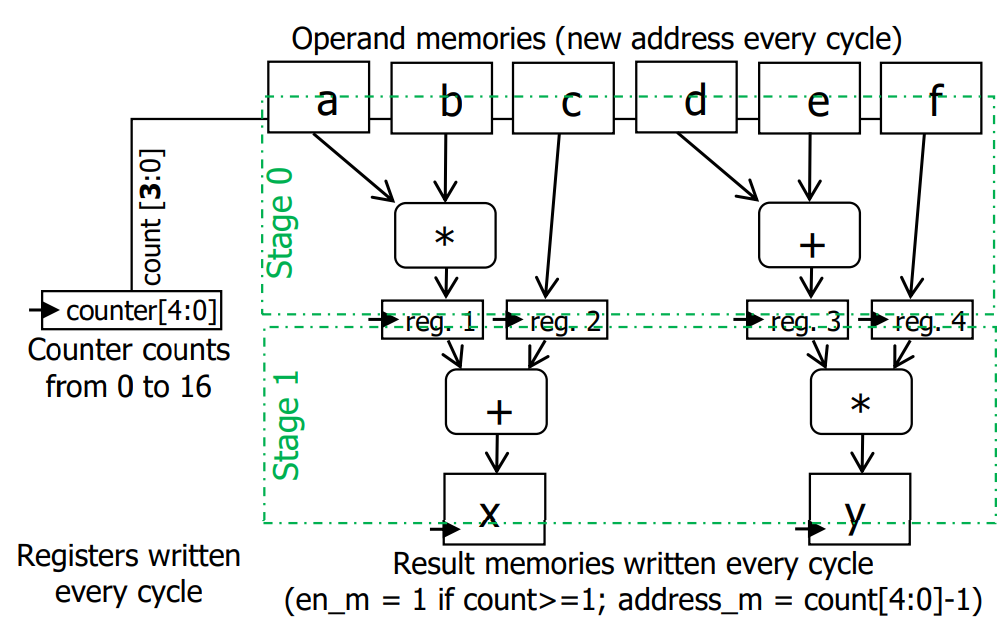
\includegraphics[width=12cm, scale=1]{S2/pipeline_II1_hardware.PNG}
    \caption{Pipeline (II=1) - Hardware implementation}
\end{figure}

\newpage
\subsection{Pipelined (\textit{II = 2})}
Issuing a new set of inputs every other cycle

\begin{itemize}
    \item In \textit{II}=1 scenario, each combinational operation was fit into one clock period, with the \textbf{slowest} combinational operation determining the fastest clock period.
    \item However, what if we could 'stretch' the \textbf{slowest} combinational operation over multiple cycles? Then we could furthur decrease the clock period.
    \item Assume that we are looking at 'stretching' the MUL operation, since it is the slowest. There are two ways to accomplish this \dots
        \begin{enumerate}[label*=\arabic*.]
            \item Modify the \textbf{combinational} MUL unit to a \textbf{sequential} one, that will now take 2 clock cycles to complete
            \item Keep the MUL unit as combinational, but manipulate the \textit{write-enable} of the registers that capture it's results.
                    This requires a \textit{set\_multicycle\_path} constraint if we were designing it manually (more in L6 - Timing Analysis)
            \begin{enumerate}[label*=\arabic*.]
                \item Combinational logic is not instantaneous in reality, there is $t_{propagation-delay}$ which denotes the maximal delay of the combinational logic.
                \item Think of it as $t_{propagation-delay} > t_{clock-period}$, therefore the write enable of the capturing register must be manipulated accordingly
            \end{enumerate}
        \end{enumerate}
\end{itemize}

\begin{minipage}[t]{0.6\textwidth}
    \vspace{0pt}
    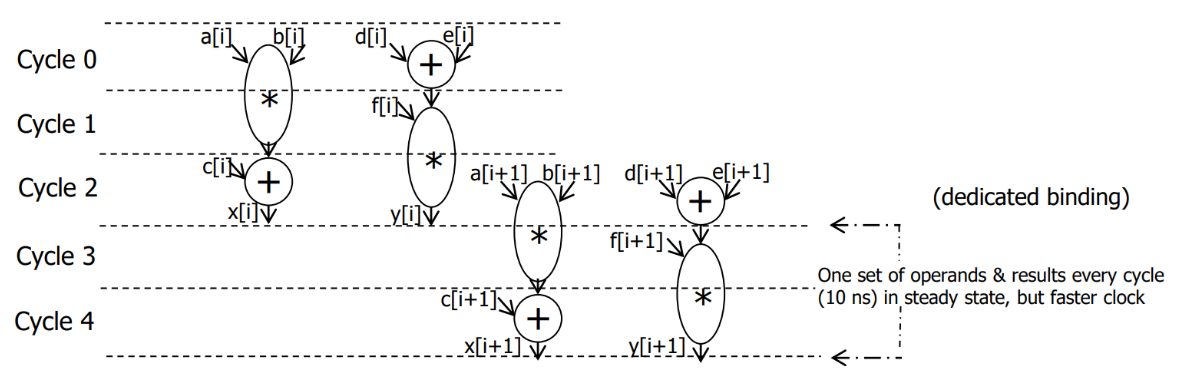
\includegraphics[width=11.5cm, scale=1]{S2/pipeline_II2_schedule.PNG}
    \captionof{figure}{Pipeline (II=2) - Scheduling}
\end{minipage}%
\begin{minipage}[t]{0.4\textwidth}
    \vspace{0pt}
    With \textit{II}=2, our clock period is 5ns and we issue a new set of inputs every 2 cycles (10ns).
    This is similar to \textit{II}=1, but our clock is operating quicker now.

    \begin{itemize}
        \item 2 ALUs, 2 MULs
        \item Period = 5ns
        \item Latency (per iteration) = 3 cycles
        \item Trip Count (number of loop iterations) = 16
        \item Total latency = (\textit{II} *tripCount) + 2 cycle overhead to fill pipeline = 34 cycles
    \end{itemize}
\end{minipage}

\begin{figure}[htp]
    \centering
    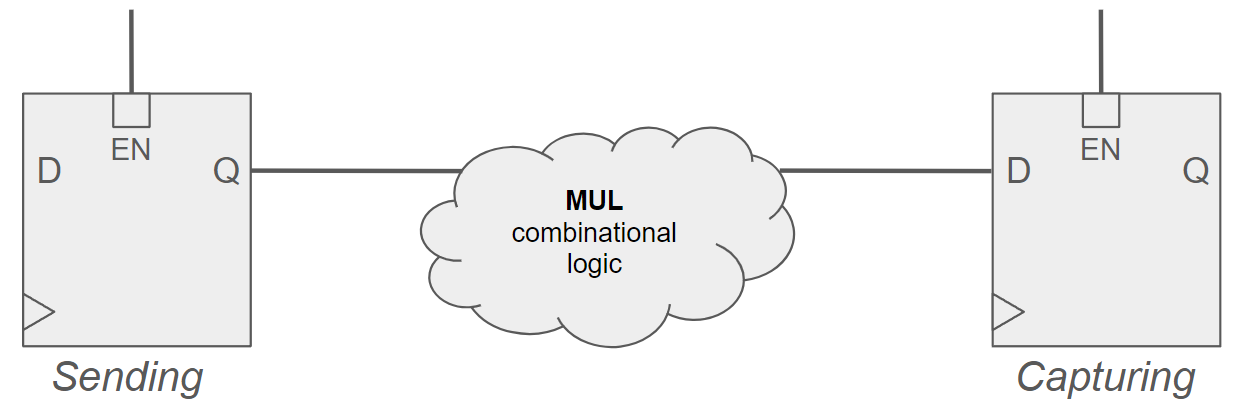
\includegraphics[width=10cm, scale=1]{S2/multLogic.PNG}
    \caption{\textit{EN} of the capturing register is asserted only on alternate clock cycles}
\end{figure}

\newpage
\begin{figure}[htp]
    \centering
    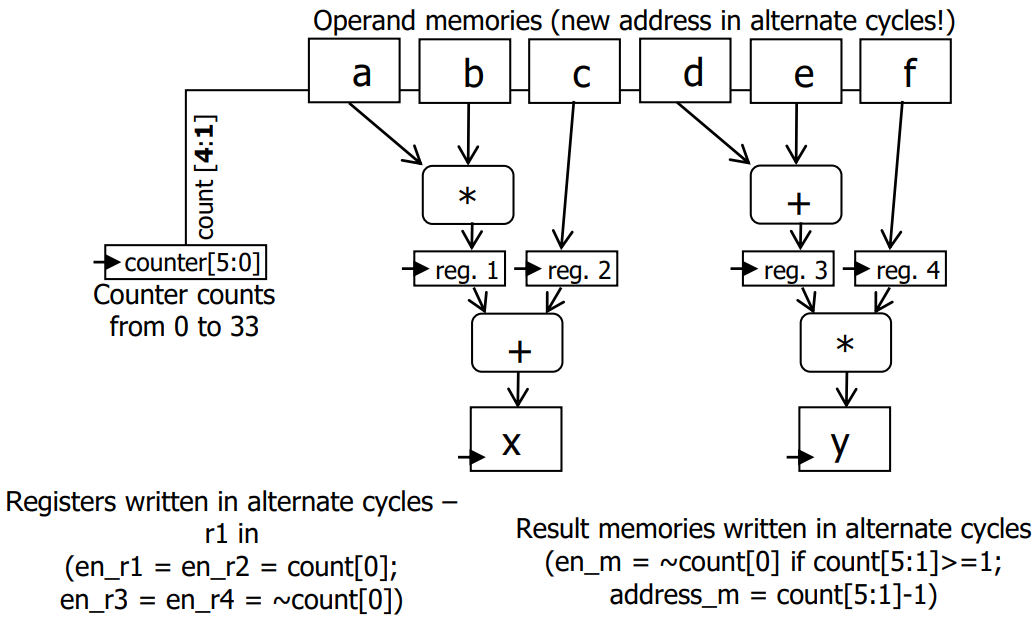
\includegraphics[width=9cm, scale=1]{S2/pipeline_II2_hardware.PNG}
    \caption{Pipeline (II=2) - Hardware implementation}
\end{figure}

\section{More aggressive optimizations}
In all the previous sections, per cycle we have at most one new input.
Is it possible to give more than one new input per cycle?

By applying some behavioral level optimizations (eg. \textit{loop unrolling}), we can.

\subsection{Loop Unrolling}
Loop unrolling requires memories that are capable of reading multiple values at a time.

In the example below for example, we would require \textit{a[i]} and \textit{a[i+1]} to be stored in seperate memories, so that they can be accessed in the same clock cycle.
One method to do so would be \textit{cyclical array partitioning} (ie. memory interleaving) by a factor of 2.

\begin{figure}[htp]
    \centering
    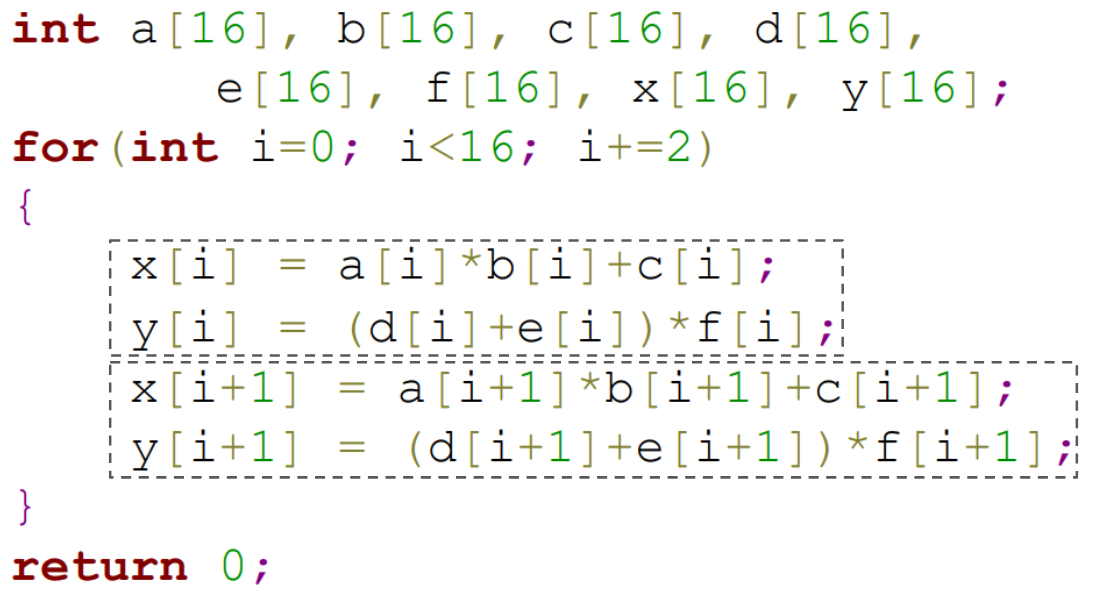
\includegraphics[width=8cm, scale=1]{S3/loopUnrolling.PNG}
    \caption{Loop unrolling by a factor of 2}
\end{figure}

\subsubsection{Unrolling + Partition + Pipelined}
\begin{figure}[htp]
    \centering
    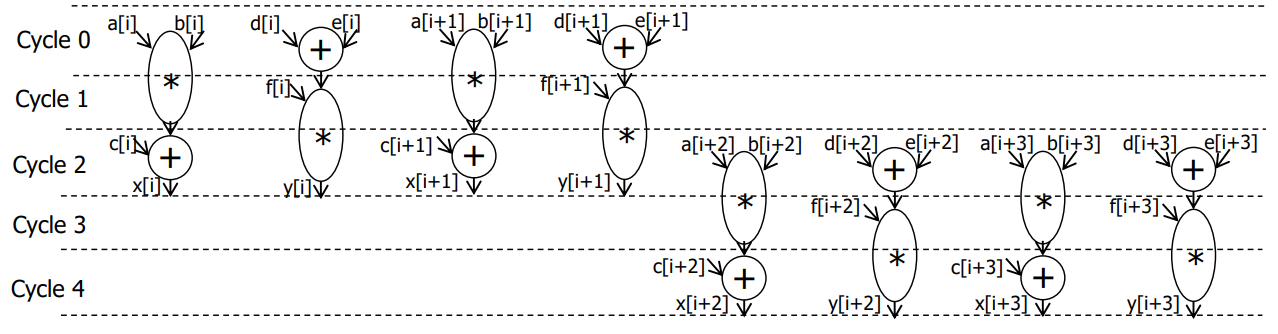
\includegraphics[width=14cm, scale=1]{S3/unrollPipelinePartition.PNG}
    \caption{Combining all optimizations together}
\end{figure}

\begin{itemize}
    \item Combining loop unrolling (by a factor of 2) and pipelining, we can give \textbf{two} sets of inputs every other cycle
    \item Note that resources will be duplicated, thus we need 4 ALUs, 4 MULs now
    \item Period = 5ns, Latency = 3 cycles, Trip count = 8 cycles
    \item Total latency = (\textit{II} *tripCount) + 2 cycle overhead to fill pipeline = 18 cycles
\end{itemize}

\end{document}